\documentclass[a4paper,11pt,titlepage]{bxjsarticle}
\usepackage[dvipdfmx]{graphicx}
\usepackage{listings}
\usepackage{amsmath}
\usepackage{fancybox,ascmac}
\usepackage{url}
\title{画像処理:第四回}
\author{175751C 宮城孝明}
\date{\today}
\begin{document}
\maketitle
\tableofcontents
\clearpage
\section{アニメ風画像加工}
\subsection{実行コード}
\lstinputlisting[language=python, numbers=left, breaklines=true, basicstyle=\ttfamily\footnotesize,
  frame=single, caption=画像風加工, label=sample]{sample.py}
  
\subsection{実行結果}
\begin{figure}[htbp]
  \begin{center}
    \begin{tabular}{c}
      % 1
      \begin{minipage}{0.33\hsize}
        \begin{center}
          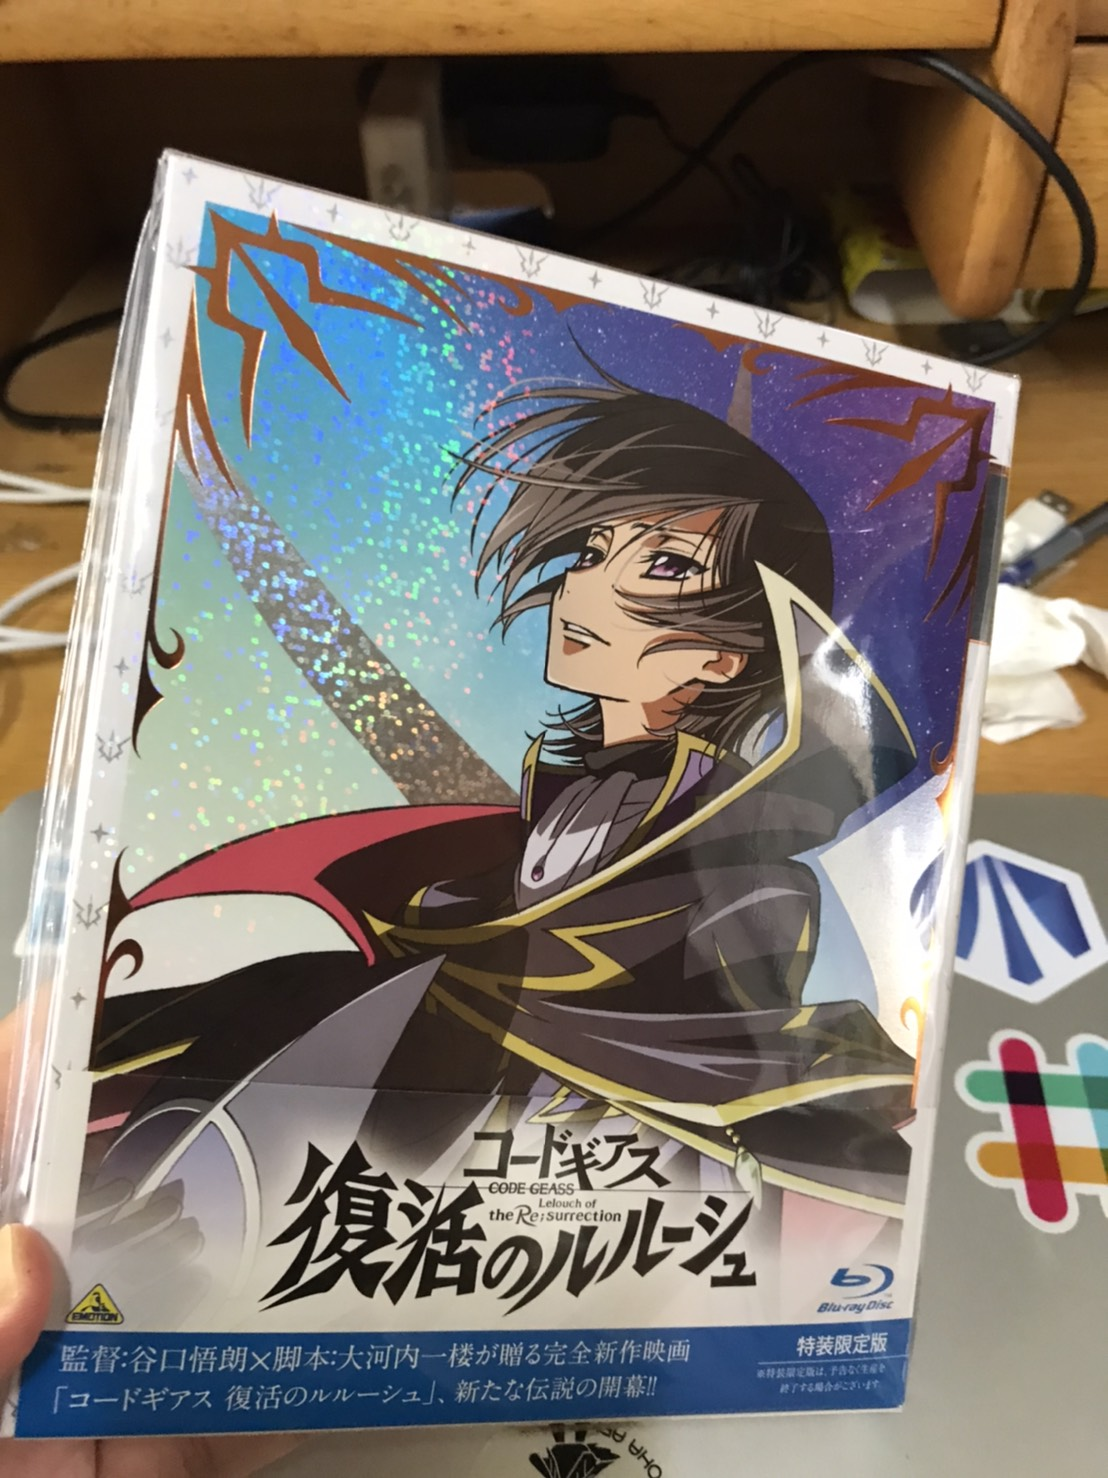
\includegraphics[clip, width=4.5cm]{./ギアス.jpg}
          \hspace{1.6cm} [1]元画像
        \end{center}
      \end{minipage}

      % 2
      \begin{minipage}{0.33\hsize}
        \begin{center}
          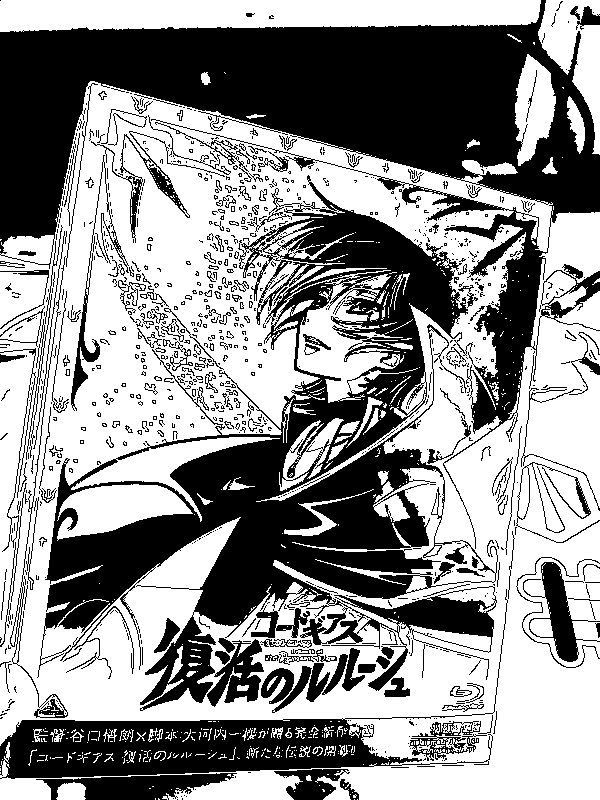
\includegraphics[clip, width=4.5cm]{./result4.jpg}
          \hspace{1.6cm} [2]結果
        \end{center}
        
      \end{minipage}
       \end{tabular}
    \caption{アニメ風加工}
    \label{fig:lena}
  \end{center}
\end{figure}
\section{}
\section{}
\begin{thebibliography}{99}
\bibitem{book1}
\bibitem{book2}
\end{thebibliography}
\end{document}


